\renewcommand{\theequation}{\theenumi}
%\subsection{Problem}

\begin{enumerate}[label=\thesubsection.\arabic*.,ref=\thesubsection.\theenumi]
\numberwithin{equation}{enumi}

\item
The following python script plots 
%
\begin{align}
f(\lambda) = a\lambda^2 + b\lambda + d
\label{eq:opt_parab}
\end{align}
%
for 
\begin{align}
a &= \norm{\vec{m}}^2 > 0
\\
b &= \vec{m}^T\brak{\vec{A} -\vec{P}} 
\\
c &= \norm{\vec{A} -\vec{P}}^2
\end{align}
where $\vec{A}$ is the intercept of the line $L$ in \eqref{eq:opt_line_nor}
on the x-axis and the points
\begin{align}
\vec{U} &= \myvec{\lambda_1\\f(\lambda_1)}, 
\vec{V} = \myvec{\lambda_2\\f(\lambda_2)}
\\
\vec{X} &= \myvec{t \lambda_1 + \brak{1-t}\lambda_2 \\ f\sbrak{t \lambda_1 + \brak{1-t}\lambda_2}},
\\
\vec{Y} &= \myvec{t \lambda_1 + \brak{1-t}\lambda_2 \\ t f\brak{\lambda_1} + \brak{1-t}f\brak{\lambda_2}}
\end{align}
%
for 
\begin{align}
\lambda_1 = -3, 
\lambda_2 = 4, 
t = 0.3
\end{align}
in Fig. \ref{fig:conv_def}. Geometrically, this means that any point $\vec{Y}$ between the points $\vec{U}, \vec{V}$ on the line $UV$ is always above the point $\vec{X}$ on the curve $f(\lambda)$.
Such a  function $f$ is defined to be {\em convex} function 
%
\begin{lstlisting}
codes/opt/1.2.py
\end{lstlisting}
%
%%
\begin{figure}[!ht]
\centering
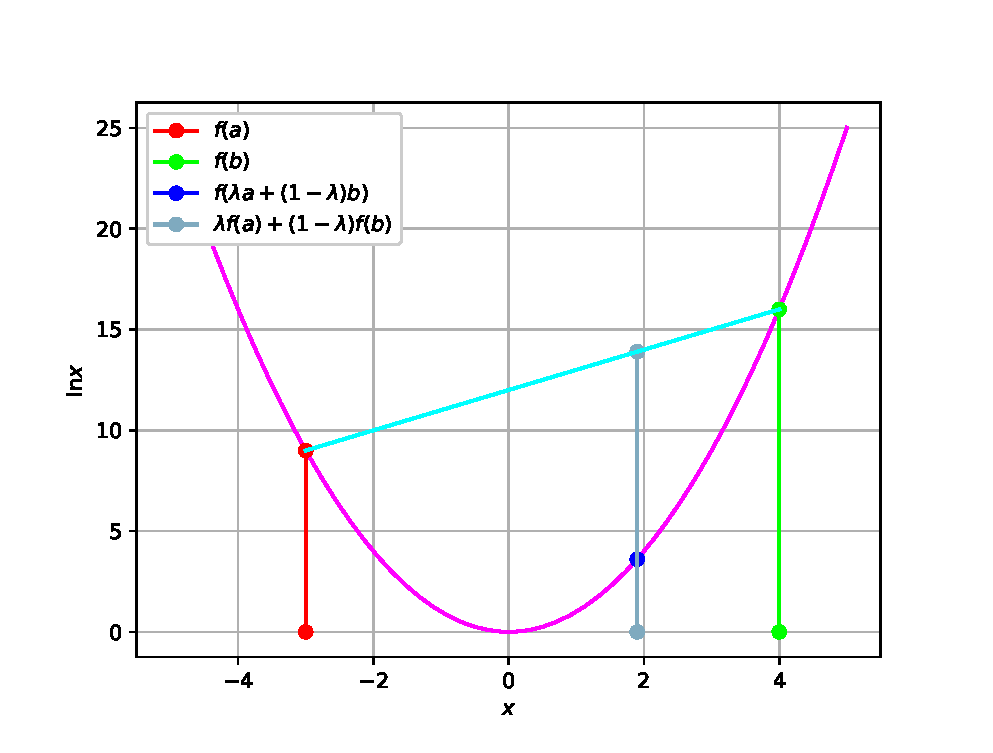
\includegraphics[width=\columnwidth]{./figs/opt/convex.eps}
\caption{ $f(\lambda)$ versus $\lambda$}.
\label{fig:conv_def}	
\end{figure}
%
\item Show that
%
\begin{align}
\label{eq:convex_def}
f\sbrak{t \lambda_1 + \brak{1-t}\lambda_2} \leq 
t f\brak{\lambda_1} + \brak{1-t}f\brak{\lambda_2}
\end{align}
%
for $\quad 0 < t < 1$.  This is true for any convex function.
%
\item Show that 
%
\begin{equation}
\eqref{eq:convex_def} \quad \implies f^{(2)}(\lambda) > 0
\end{equation}
%
\item Show that a covex function has a unique minimum.
%
\end{enumerate}
%
